\documentclass{standalone}
\usepackage{tikz}
\usetikzlibrary{patterns, positioning}
\usepackage[sfdefault]{ClearSans} %% option 'sfdefault' activates Clear Sans as the default text font
\usepackage[T1]{fontenc}

\begin{document}
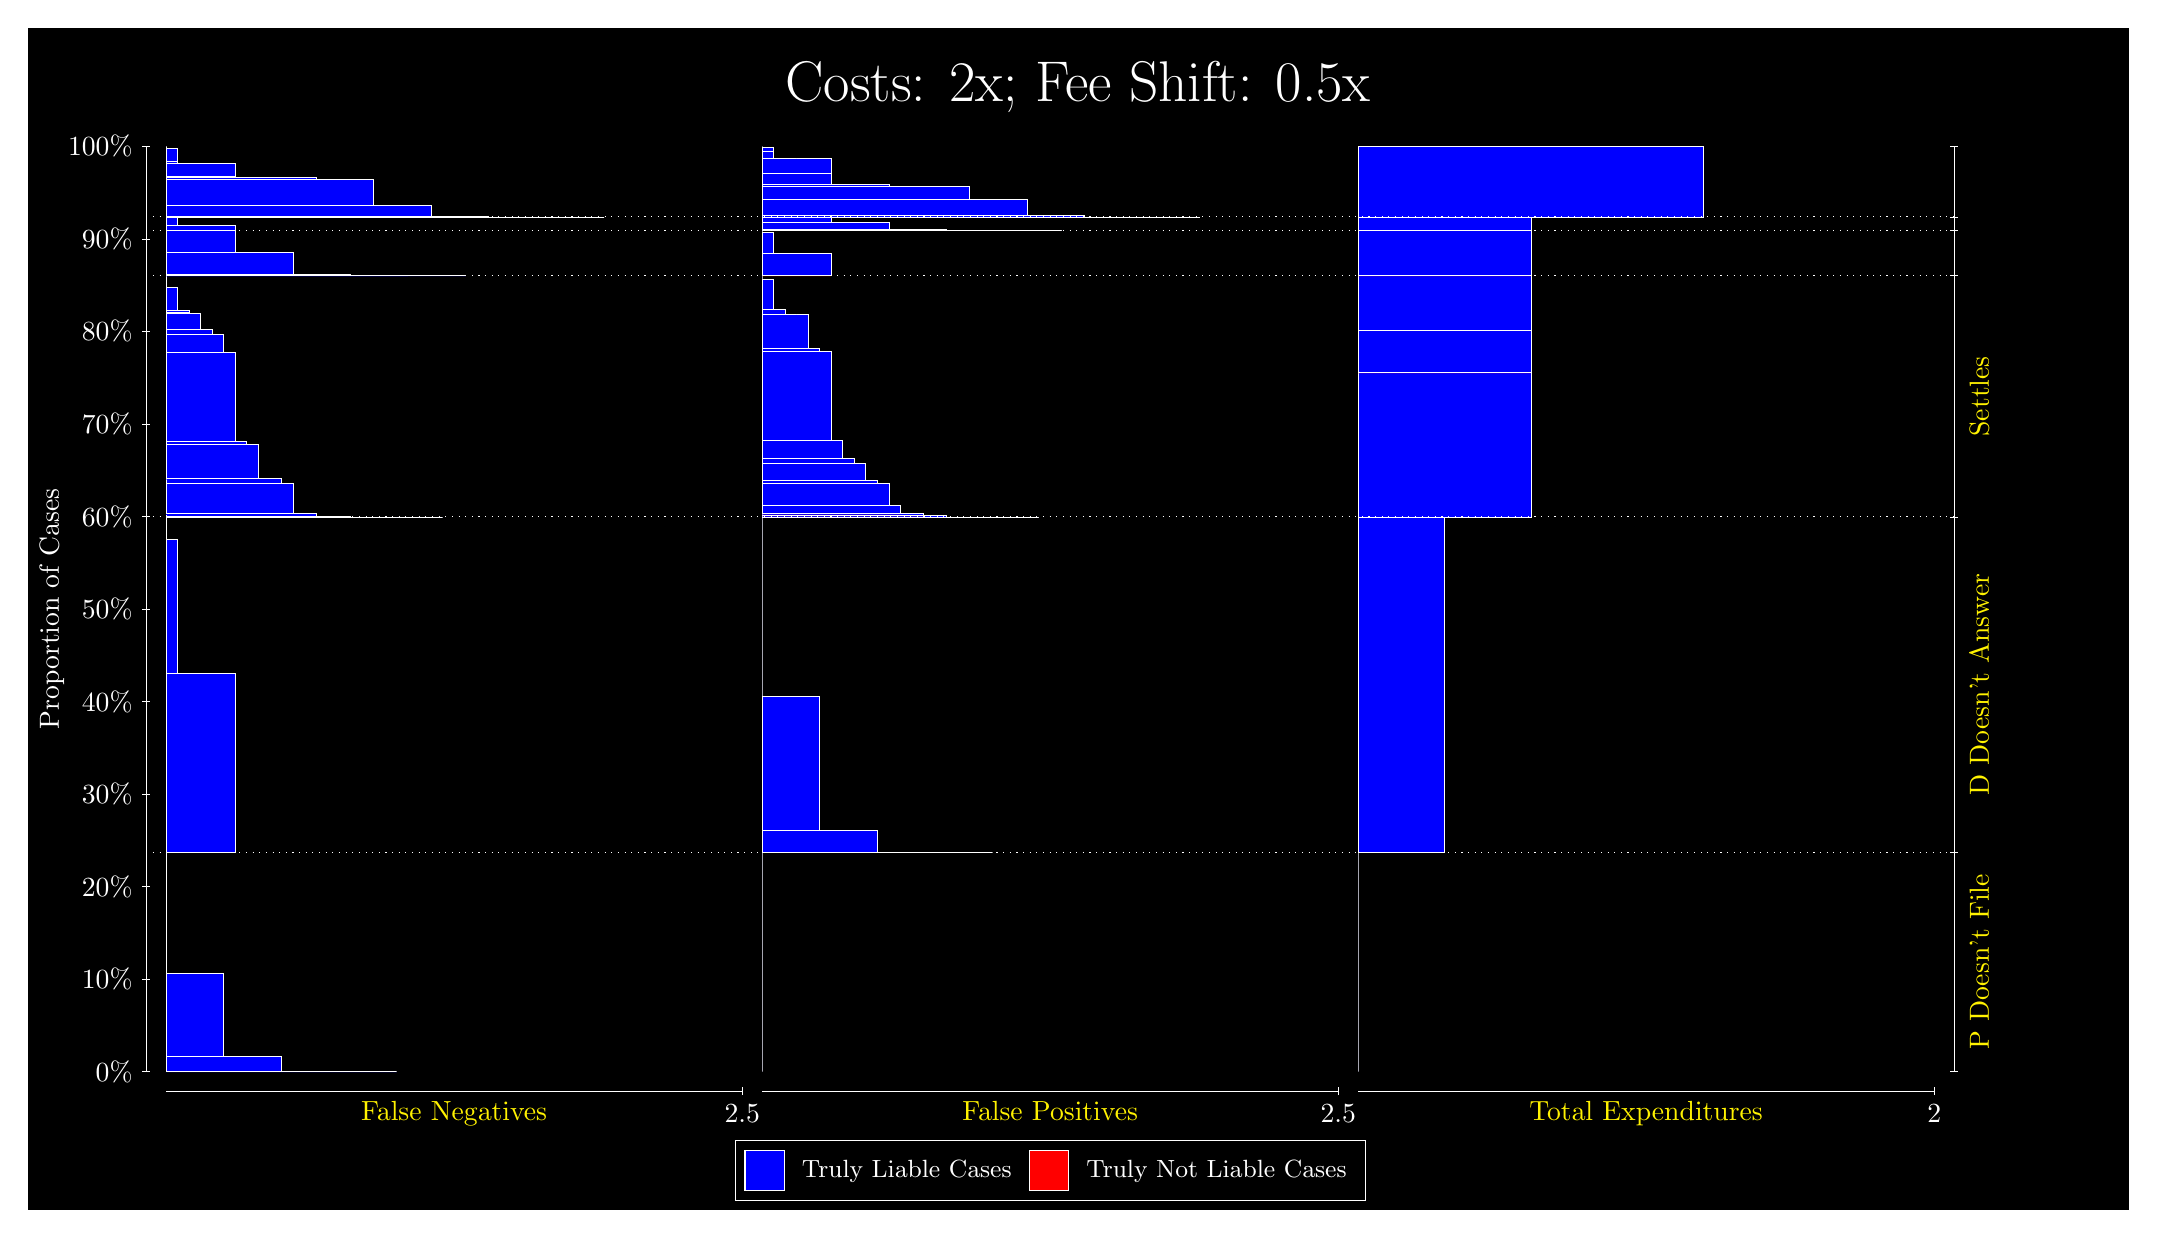
\begin{tikzpicture}
\draw[fill=black] (0,0) rectangle (26.667,15);
\draw[text=white] (0,13.5) rectangle (26.667,15) node[midway] {\huge Costs: 2x; Fee Shift: 0.5x};
\draw[white, very thin] (1.5,1.75) -- (1.5,13.5);
\node[rotate=90, text=white, anchor=center] at (0.3, 7.625) {Proportion of Cases};
\draw[white, very thin] (1.45,1.75) -- (1.55,1.75);
\node[text=white, anchor=east] at (1.45, 1.75) {0\%};
\draw[white, very thin] (1.45,2.925) -- (1.55,2.925);
\node[text=white, anchor=east] at (1.45, 2.925) {10\%};
\draw[white, very thin] (1.45,4.1) -- (1.55,4.1);
\node[text=white, anchor=east] at (1.45, 4.1) {20\%};
\draw[white, very thin] (1.45,5.275) -- (1.55,5.275);
\node[text=white, anchor=east] at (1.45, 5.275) {30\%};
\draw[white, very thin] (1.45,6.45) -- (1.55,6.45);
\node[text=white, anchor=east] at (1.45, 6.45) {40\%};
\draw[white, very thin] (1.45,7.625) -- (1.55,7.625);
\node[text=white, anchor=east] at (1.45, 7.625) {50\%};
\draw[white, very thin] (1.45,8.8) -- (1.55,8.8);
\node[text=white, anchor=east] at (1.45, 8.8) {60\%};
\draw[white, very thin] (1.45,9.975) -- (1.55,9.975);
\node[text=white, anchor=east] at (1.45, 9.975) {70\%};
\draw[white, very thin] (1.45,11.15) -- (1.55,11.15);
\node[text=white, anchor=east] at (1.45, 11.15) {80\%};
\draw[white, very thin] (1.45,12.325) -- (1.55,12.325);
\node[text=white, anchor=east] at (1.45, 12.325) {90\%};
\draw[white, very thin] (1.45,13.5) -- (1.55,13.5);
\node[text=white, anchor=east] at (1.45, 13.5) {100\%};

\draw[white, very thin] (24.457,1.75) -- (24.457,13.5);
\draw[white, very thin] (24.407,1.75) -- (24.507,1.75);
\node[anchor=west] at (24.407, 1.75) {};
\draw[white, very thin] (24.407,4.5319) -- (24.507,4.5319);
\node[anchor=west] at (24.407, 4.5319) {};
\draw[white, very thin] (24.407,8.7937) -- (24.507,8.7937);
\node[anchor=west] at (24.407, 8.7937) {};
\draw[white, very thin] (24.407,11.857) -- (24.507,11.857);
\node[anchor=west] at (24.407, 11.857) {};
\draw[white, very thin] (24.407,12.434) -- (24.507,12.434);
\node[anchor=west] at (24.407, 12.434) {};
\draw[white, very thin] (24.407,12.604) -- (24.507,12.604);
\node[anchor=west] at (24.407, 12.604) {};
\draw[white, very thin] (24.407,13.5) -- (24.507,13.5);
\node[anchor=west] at (24.407, 13.5) {};

\draw[white, very thin, fill=blue] (1.75,1.75) rectangle (4.6775,1.75);
\draw[white, very thin, fill=blue] (1.75,1.75) rectangle (3.9457,1.7516);
\draw[white, very thin, fill=blue] (1.75,1.7516) rectangle (3.2138,1.9394);
\draw[white, very thin, fill=blue] (1.75,1.9394) rectangle (2.4819,3.0004);
\draw[white, very thin, fill=red] (1.75,3.0004) rectangle (1.75,3.0004);
\draw[white, very thin, fill=blue] (1.75,3.0004) rectangle (1.75,4.5319);
\draw[white, very thin, fill=blue] (1.75,4.5319) rectangle (2.6283,6.8036);
\draw[white, very thin, fill=blue] (1.75,6.8036) rectangle (1.8964,8.5069);
\draw[white, very thin, fill=red] (1.75,8.5069) rectangle (1.75,8.5069);
\draw[white, very thin, fill=blue] (1.75,8.5069) rectangle (1.75,8.7937);
\draw[white, very thin, fill=blue] (1.75,8.7937) rectangle (5.2631,8.7937);
\draw[white, very thin, fill=blue] (1.75,8.7937) rectangle (4.9703,8.7937);
\draw[white, very thin, fill=blue] (1.75,8.7937) rectangle (4.6775,8.7937);
\draw[white, very thin, fill=blue] (1.75,8.7937) rectangle (4.5312,8.7937);
\draw[white, very thin, fill=blue] (1.75,8.7937) rectangle (4.3848,8.7937);
\draw[white, very thin, fill=blue] (1.75,8.7937) rectangle (4.3848,8.7937);
\draw[white, very thin, fill=blue] (1.75,8.7937) rectangle (4.2384,8.7937);
\draw[white, very thin, fill=blue] (1.75,8.7937) rectangle (4.092,8.8042);
\draw[white, very thin, fill=blue] (1.75,8.8042) rectangle (3.9457,8.8044);
\draw[white, very thin, fill=blue] (1.75,8.8044) rectangle (3.7993,8.8044);
\draw[white, very thin, fill=blue] (1.75,8.8044) rectangle (3.6529,8.8044);
\draw[white, very thin, fill=blue] (1.75,8.8044) rectangle (3.6529,8.8351);
\draw[white, very thin, fill=blue] (1.75,8.8351) rectangle (3.5065,8.8351);
\draw[white, very thin, fill=blue] (1.75,8.8351) rectangle (3.5065,8.8364);
\draw[white, very thin, fill=blue] (1.75,8.8364) rectangle (3.3602,9.2191);
\draw[white, very thin, fill=blue] (1.75,9.2191) rectangle (3.2138,9.279);
\draw[white, very thin, fill=blue] (1.75,9.279) rectangle (3.0674,9.2792);
\draw[white, very thin, fill=blue] (1.75,9.2792) rectangle (3.0674,9.2889);
\draw[white, very thin, fill=blue] (1.75,9.2889) rectangle (2.921,9.2889);
\draw[white, very thin, fill=blue] (1.75,9.2889) rectangle (2.921,9.7177);
\draw[white, very thin, fill=blue] (1.75,9.7177) rectangle (2.921,9.7178);
\draw[white, very thin, fill=blue] (1.75,9.7178) rectangle (2.7746,9.7179);
\draw[white, very thin, fill=blue] (1.75,9.7179) rectangle (2.7746,9.753);
\draw[white, very thin, fill=blue] (1.75,9.753) rectangle (2.6283,10.889);
\draw[white, very thin, fill=blue] (1.75,10.889) rectangle (2.4819,11.11);
\draw[white, very thin, fill=blue] (1.75,11.11) rectangle (2.3355,11.111);
\draw[white, very thin, fill=blue] (1.75,11.111) rectangle (2.3355,11.178);
\draw[white, very thin, fill=blue] (1.75,11.178) rectangle (2.1891,11.178);
\draw[white, very thin, fill=blue] (1.75,11.178) rectangle (2.1891,11.386);
\draw[white, very thin, fill=blue] (1.75,11.386) rectangle (2.1891,11.386);
\draw[white, very thin, fill=blue] (1.75,11.386) rectangle (2.0428,11.387);
\draw[white, very thin, fill=blue] (1.75,11.387) rectangle (2.0428,11.424);
\draw[white, very thin, fill=blue] (1.75,11.424) rectangle (1.8964,11.711);
\draw[white, very thin, fill=red] (1.75,11.711) rectangle (1.75,11.711);
\draw[white, very thin, fill=blue] (1.75,11.711) rectangle (1.75,11.857);
\draw[white, very thin, fill=blue] (1.75,11.857) rectangle (5.5558,11.857);
\draw[white, very thin, fill=blue] (1.75,11.857) rectangle (4.8239,11.857);
\draw[white, very thin, fill=blue] (1.75,11.857) rectangle (4.092,11.877);
\draw[white, very thin, fill=blue] (1.75,11.877) rectangle (3.3602,12.151);
\draw[white, very thin, fill=blue] (1.75,12.151) rectangle (2.6283,12.434);
\draw[white, very thin, fill=red] (1.75,12.434) rectangle (1.75,12.434);
\draw[white, very thin, fill=blue] (1.75,12.434) rectangle (2.6283,12.498);
\draw[white, very thin, fill=blue] (1.75,12.498) rectangle (1.8964,12.596);
\draw[white, very thin, fill=red] (1.75,12.596) rectangle (1.75,12.596);
\draw[white, very thin, fill=blue] (1.75,12.596) rectangle (1.75,12.604);
\draw[white, very thin, fill=blue] (1.75,12.604) rectangle (7.3123,12.604);
\draw[white, very thin, fill=blue] (1.75,12.604) rectangle (6.5805,12.604);
\draw[white, very thin, fill=blue] (1.75,12.604) rectangle (5.8486,12.612);
\draw[white, very thin, fill=blue] (1.75,12.612) rectangle (5.1167,12.753);
\draw[white, very thin, fill=blue] (1.75,12.753) rectangle (4.8239,12.753);
\draw[white, very thin, fill=blue] (1.75,12.753) rectangle (4.3848,13.081);
\draw[white, very thin, fill=blue] (1.75,13.081) rectangle (4.092,13.081);
\draw[white, very thin, fill=blue] (1.75,13.081) rectangle (3.6529,13.11);
\draw[white, very thin, fill=blue] (1.75,13.11) rectangle (3.3602,13.112);
\draw[white, very thin, fill=blue] (1.75,13.112) rectangle (2.921,13.112);
\draw[white, very thin, fill=blue] (1.75,13.112) rectangle (2.6283,13.114);
\draw[white, very thin, fill=blue] (1.75,13.114) rectangle (2.6283,13.28);
\draw[white, very thin, fill=blue] (1.75,13.28) rectangle (1.8964,13.311);
\draw[white, very thin, fill=blue] (1.75,13.311) rectangle (1.8964,13.481);
\draw[white, very thin, fill=red] (1.75,13.481) rectangle (1.75,13.481);
\draw[white, very thin, fill=blue] (1.75,13.481) rectangle (1.75,13.5);
\draw[white, very thin, fill=red] (9.3189,1.75) rectangle (9.3189,1.75);
\draw[white, very thin, fill=blue] (9.3189,1.75) rectangle (9.3189,4.5319);
\draw[white, very thin, fill=red] (9.3189,4.5319) rectangle (12.246,4.5319);
\draw[white, very thin, fill=blue] (9.3189,4.5319) rectangle (12.246,4.5319);
\draw[white, very thin, fill=blue] (9.3189,4.5319) rectangle (11.515,4.5334);
\draw[white, very thin, fill=blue] (9.3189,4.5334) rectangle (10.783,4.8188);
\draw[white, very thin, fill=blue] (9.3189,4.8188) rectangle (10.051,6.522);
\draw[white, very thin, fill=blue] (9.3189,6.522) rectangle (9.3189,8.7937);
\draw[white, very thin, fill=red] (9.3189,8.7937) rectangle (12.832,8.7937);
\draw[white, very thin, fill=blue] (9.3189,8.7937) rectangle (12.832,8.7937);
\draw[white, very thin, fill=red] (9.3189,8.7937) rectangle (12.539,8.7937);
\draw[white, very thin, fill=blue] (9.3189,8.7937) rectangle (12.539,8.7937);
\draw[white, very thin, fill=red] (9.3189,8.7937) rectangle (12.246,8.7937);
\draw[white, very thin, fill=blue] (9.3189,8.7937) rectangle (12.246,8.7937);
\draw[white, very thin, fill=blue] (9.3189,8.7937) rectangle (12.1,8.7937);
\draw[white, very thin, fill=red] (9.3189,8.7937) rectangle (11.954,8.7937);
\draw[white, very thin, fill=blue] (9.3189,8.7937) rectangle (11.954,8.7937);
\draw[white, very thin, fill=blue] (9.3189,8.7937) rectangle (11.807,8.7937);
\draw[white, very thin, fill=red] (9.3189,8.7937) rectangle (11.661,8.7937);
\draw[white, very thin, fill=blue] (9.3189,8.7937) rectangle (11.661,8.8104);
\draw[white, very thin, fill=blue] (9.3189,8.8104) rectangle (11.515,8.8105);
\draw[white, very thin, fill=red] (9.3189,8.8105) rectangle (11.368,8.8105);
\draw[white, very thin, fill=blue] (9.3189,8.8105) rectangle (11.368,8.836);
\draw[white, very thin, fill=blue] (9.3189,8.836) rectangle (11.222,8.8362);
\draw[white, very thin, fill=blue] (9.3189,8.8362) rectangle (11.075,8.8362);
\draw[white, very thin, fill=red] (9.3189,8.8362) rectangle (11.075,8.8362);
\draw[white, very thin, fill=blue] (9.3189,8.8362) rectangle (11.075,8.9397);
\draw[white, very thin, fill=blue] (9.3189,8.9397) rectangle (10.929,9.2266);
\draw[white, very thin, fill=red] (9.3189,9.2266) rectangle (10.783,9.2266);
\draw[white, very thin, fill=blue] (9.3189,9.2266) rectangle (10.783,9.264);
\draw[white, very thin, fill=blue] (9.3189,9.264) rectangle (10.636,9.472);
\draw[white, very thin, fill=red] (9.3189,9.472) rectangle (10.49,9.472);
\draw[white, very thin, fill=blue] (9.3189,9.472) rectangle (10.49,9.5391);
\draw[white, very thin, fill=blue] (9.3189,9.5391) rectangle (10.49,9.5402);
\draw[white, very thin, fill=blue] (9.3189,9.5402) rectangle (10.344,9.5402);
\draw[white, very thin, fill=blue] (9.3189,9.5402) rectangle (10.344,9.7616);
\draw[white, very thin, fill=blue] (9.3189,9.7616) rectangle (10.197,10.897);
\draw[white, very thin, fill=blue] (9.3189,10.897) rectangle (10.051,10.933);
\draw[white, very thin, fill=blue] (9.3189,10.933) rectangle (9.9044,11.362);
\draw[white, very thin, fill=blue] (9.3189,11.362) rectangle (9.758,11.371);
\draw[white, very thin, fill=blue] (9.3189,11.371) rectangle (9.758,11.371);
\draw[white, very thin, fill=blue] (9.3189,11.371) rectangle (9.6116,11.371);
\draw[white, very thin, fill=blue] (9.3189,11.371) rectangle (9.6116,11.431);
\draw[white, very thin, fill=blue] (9.3189,11.431) rectangle (9.4652,11.814);
\draw[white, very thin, fill=blue] (9.3189,11.814) rectangle (9.3189,11.857);
\draw[white, very thin, fill=red] (9.3189,11.857) rectangle (10.197,11.857);
\draw[white, very thin, fill=blue] (9.3189,11.857) rectangle (10.197,12.139);
\draw[white, very thin, fill=blue] (9.3189,12.139) rectangle (9.4652,12.414);
\draw[white, very thin, fill=blue] (9.3189,12.414) rectangle (9.3189,12.434);
\draw[white, very thin, fill=red] (9.3189,12.434) rectangle (13.125,12.434);
\draw[white, very thin, fill=blue] (9.3189,12.434) rectangle (13.125,12.434);
\draw[white, very thin, fill=blue] (9.3189,12.434) rectangle (12.393,12.434);
\draw[white, very thin, fill=blue] (9.3189,12.434) rectangle (11.661,12.441);
\draw[white, very thin, fill=blue] (9.3189,12.441) rectangle (10.929,12.539);
\draw[white, very thin, fill=blue] (9.3189,12.539) rectangle (10.197,12.604);
\draw[white, very thin, fill=red] (9.3189,12.604) rectangle (14.881,12.604);
\draw[white, very thin, fill=blue] (9.3189,12.604) rectangle (14.881,12.604);
\draw[white, very thin, fill=red] (9.3189,12.604) rectangle (14.149,12.604);
\draw[white, very thin, fill=blue] (9.3189,12.604) rectangle (14.149,12.604);
\draw[white, very thin, fill=red] (9.3189,12.604) rectangle (13.417,12.604);
\draw[white, very thin, fill=blue] (9.3189,12.604) rectangle (13.417,12.623);
\draw[white, very thin, fill=red] (9.3189,12.623) rectangle (12.686,12.623);
\draw[white, very thin, fill=blue] (9.3189,12.623) rectangle (12.686,12.824);
\draw[white, very thin, fill=blue] (9.3189,12.824) rectangle (11.954,12.992);
\draw[white, very thin, fill=red] (9.3189,12.992) rectangle (11.661,12.992);
\draw[white, very thin, fill=blue] (9.3189,12.992) rectangle (11.661,12.992);
\draw[white, very thin, fill=blue] (9.3189,12.992) rectangle (11.222,12.994);
\draw[white, very thin, fill=red] (9.3189,12.994) rectangle (10.929,12.994);
\draw[white, very thin, fill=blue] (9.3189,12.994) rectangle (10.929,13.023);
\draw[white, very thin, fill=blue] (9.3189,13.023) rectangle (10.49,13.023);
\draw[white, very thin, fill=blue] (9.3189,13.023) rectangle (10.197,13.162);
\draw[white, very thin, fill=red] (9.3189,13.162) rectangle (10.197,13.162);
\draw[white, very thin, fill=blue] (9.3189,13.162) rectangle (10.197,13.351);
\draw[white, very thin, fill=blue] (9.3189,13.351) rectangle (9.758,13.351);
\draw[white, very thin, fill=blue] (9.3189,13.351) rectangle (9.4652,13.433);
\draw[white, very thin, fill=blue] (9.3189,13.433) rectangle (9.4652,13.492);
\draw[white, very thin, fill=blue] (9.3189,13.492) rectangle (9.3189,13.5);
\draw[white, very thin, fill=red] (16.888,1.75) rectangle (16.888,1.75);
\draw[white, very thin, fill=blue] (16.888,1.75) rectangle (16.888,4.5319);
\draw[white, very thin, fill=red] (16.888,4.5319) rectangle (17.986,4.5319);
\draw[white, very thin, fill=blue] (16.888,4.5319) rectangle (17.986,8.7937);
\draw[white, very thin, fill=red] (16.888,8.7937) rectangle (19.083,8.7937);
\draw[white, very thin, fill=blue] (16.888,8.7937) rectangle (19.083,10.627);
\draw[white, very thin, fill=red] (16.888,10.627) rectangle (19.083,10.627);
\draw[white, very thin, fill=blue] (16.888,10.627) rectangle (19.083,11.162);
\draw[white, very thin, fill=red] (16.888,11.162) rectangle (19.083,11.162);
\draw[white, very thin, fill=blue] (16.888,11.162) rectangle (19.083,11.857);
\draw[white, very thin, fill=red] (16.888,11.857) rectangle (19.083,11.857);
\draw[white, very thin, fill=blue] (16.888,11.857) rectangle (19.083,12.434);
\draw[white, very thin, fill=red] (16.888,12.434) rectangle (19.083,12.434);
\draw[white, very thin, fill=blue] (16.888,12.434) rectangle (19.083,12.604);
\draw[white, very thin, fill=red] (16.888,12.604) rectangle (21.279,12.604);
\draw[white, very thin, fill=blue] (16.888,12.604) rectangle (21.279,13.5);
\draw[white, dotted] (1.5,4.5319) -- (24.457,4.5319);
\draw[white, dotted] (1.5,8.7937) -- (24.457,8.7937);
\draw[white, dotted] (1.5,11.857) -- (24.457,11.857);
\draw[white, dotted] (1.5,12.434) -- (24.457,12.434);
\draw[white, dotted] (1.5,12.604) -- (24.457,12.604);
\draw[white, very thin] (1.75,1.5) -- (9.0689,1.5);
\node[text=yellow, anchor=north] at (5.4094, 1.5) {False Negatives};
\draw[white, very thin] (9.0689,1.45) -- (9.0689,1.55);
\node[text=white, anchor=north] at (9.0689, 1.45) {2.5};

\draw[white, very thin] (9.3189,1.5) -- (16.638,1.5);
\node[text=yellow, anchor=north] at (12.978, 1.5) {False Positives};
\draw[white, very thin] (16.638,1.45) -- (16.638,1.55);
\node[text=white, anchor=north] at (16.638, 1.45) {2.5};

\draw[white, very thin] (16.888,1.5) -- (24.207,1.5);
\node[text=yellow, anchor=north] at (20.547, 1.5) {Total Expenditures};
\draw[white, very thin] (24.207,1.45) -- (24.207,1.55);
\node[text=white, anchor=north] at (24.207, 1.45) {2};

\node[text=yellow, centered, rotate=90] at (24.777, 3.141) {P Doesn't File};
\node[text=yellow, centered, rotate=90] at (24.777, 6.6628) {D Doesn't Answer};
\node[text=yellow, centered, rotate=90] at (24.777, 10.325) {Settles};




\draw (12.978300999999998,1.5) node[draw=none] (baseCoordinate) {};
\begin{scope}[align=center]
        \matrix[scale=0.5, draw=white, below=0.5cm of baseCoordinate, nodes={draw}, column sep=0.1cm]{
            \node[rectangle, draw, minimum width=0.5cm, minimum height=0.5cm, fill=blue] {}; &
            \node[draw=none, font=\small, text=white] (B) {Truly Liable Cases}; &
            \node[rectangle, draw, minimum width=0.5cm, minimum height=0.5cm, fill=red] {}; &
            \node[draw=none, font=\small, text=white] (B) {Truly Not Liable Cases}; \\
            };
\end{scope}

\end{tikzpicture}
\end{document}